\subsection{Señalamiento original}

	El señalamiento original, ilustrado en la Figura \ref{fig:EJ9_2}, no incluye señales al ser un ejemplo de diseño de una red ferroviaria para una locación real, de la cual no fue proporcionada ninguna información salvo la topología de la red. El objetivo de este ejemplo fue comparar el señalamiento generado sin tener ninguna otra referencia externa.
	
	\begin{figure}[H]
		\centering
		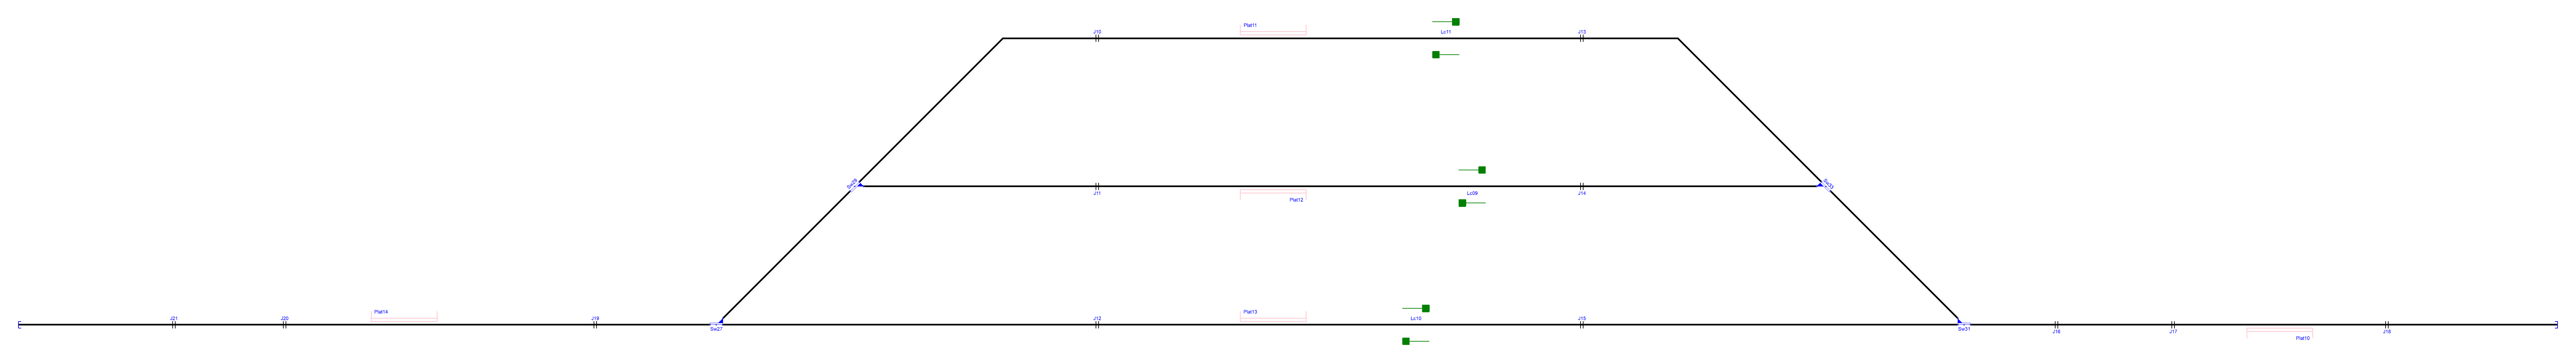
\includegraphics[width=1\textwidth]{resultados-obtenidos/ejemplo9/images/9_original.png}
		\centering\caption{Señalamiento original del ejemplo 9.}
		\label{fig:EJ9_2}
	\end{figure}
	
	La cantidad de rutas existentes es indefinida, así como también el sentido de circulación de las vías.